\subsection{Test af EMG}

EMG-forstærkeren testes for at vurdere, hvorvidt muskelsignalerne fra rectus femoris opsamles. Elektoderne placeres midt for linjen mellem anterior spina iliaca superior og den superior del af patella ud fra SENIAM's anvisning om elektrodeplacering. En squat-øvelse udføres, mens muskelsignaler opsamles i MATLAB. Muskelsignalet under udførelsen af squat-øvelsen fremgår af \autoref{fig:raat_emg} 

\begin{figure}[H]
\centering
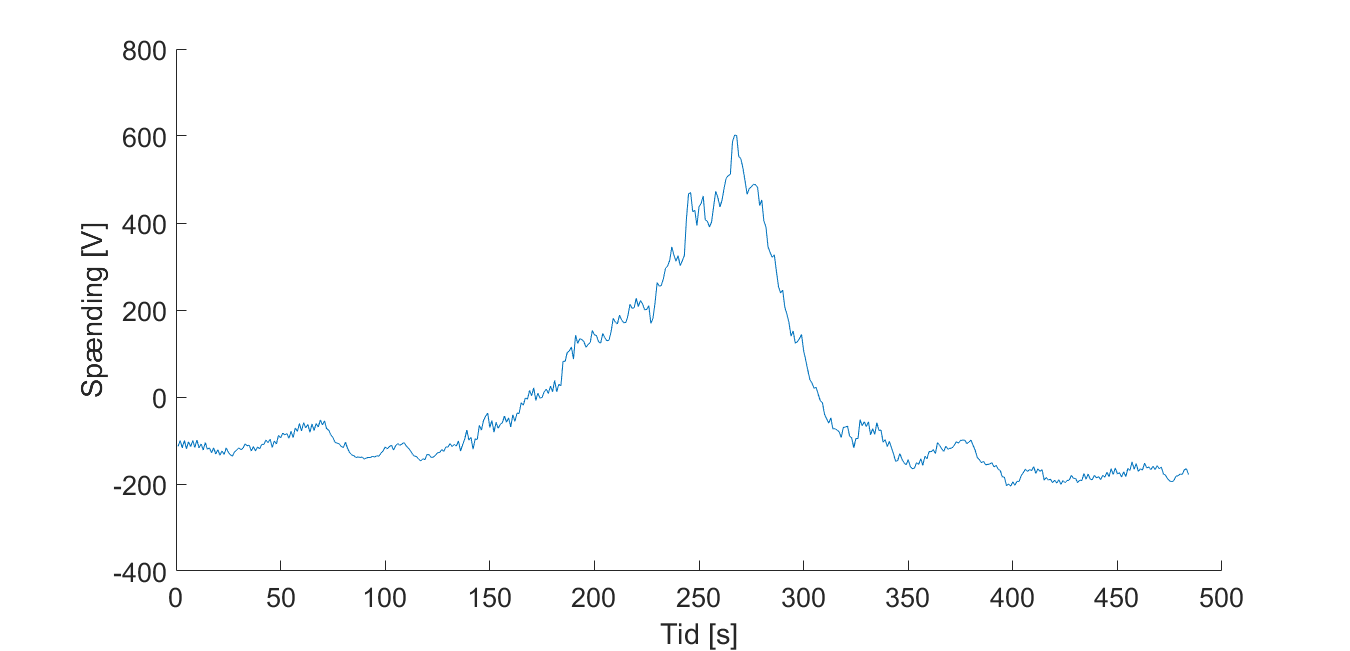
\includegraphics[width=0.8\textwidth]{figures/raat_EMG_test}
\caption{Et ufiltreret EMG-signal fra rectus femoris under udførsel af en squat-øvelse}
\label{fig:raat_emg}
\end{figure}

\subsection{Test af accelerometer}

Accelerometrene testet for at vurdere, hvorvidt de opstillede krav opfyldes. Der tages udgangspunkt i værdierne fra databladet for ADXL335, da det ikke er muligt at teste alle opstillede krav. Accelerometrene kan forsynes med en DC-forsyning fra $1,8-3,6 V$. Da accelerometrene skal kunne forsynes med en spænding på $3,3 V$, opfyldes dette krav. Herudover ses det ud fra databladet, at der er en linearitet med en afvigelse på $0,3\%$ samt et lineært arbejdsområde på $ \pm 3 g$. Af databladet fremgår det ligeledes, at accelerometrene er triaksiale. Det er derfor muligt at måle på minimum én akse.  

